\documentclass{article}
\usepackage[T1]{fontenc}
\usepackage{lmodern}
\usepackage{graphicx}
\usepackage{amsmath,amssymb}
\usepackage[a4paper,margin=2cm]{geometry}
\usepackage[absolute,overlay]{textpos}
\setlength{\TPHorizModule}{1mm}
\setlength{\TPVertModule}{1mm}
\usepackage[indonesian]{babel}
\usepackage{hyperref}
\setlength{\emergencystretch}{2em}
% unit: Halaman 8

\begin{document}

% === Halaman 8 (llm) ===

\vspace{246.51mm}

Konversi biner ke hex:

% deskripsi: Screenshot alat konversi biner ke heksadesimal dari situs RapidTables yang menunjukkan konversi bilangan biner 110101010111000101 menjadi heksadesimal D5C5 dan desimal 54725.
% bbox normalisasi: [0.0700, 0.1100, 0.9400, 0.9400]
\begin{textblock*}{182.70mm}(14.70mm,32.67mm)
\noindent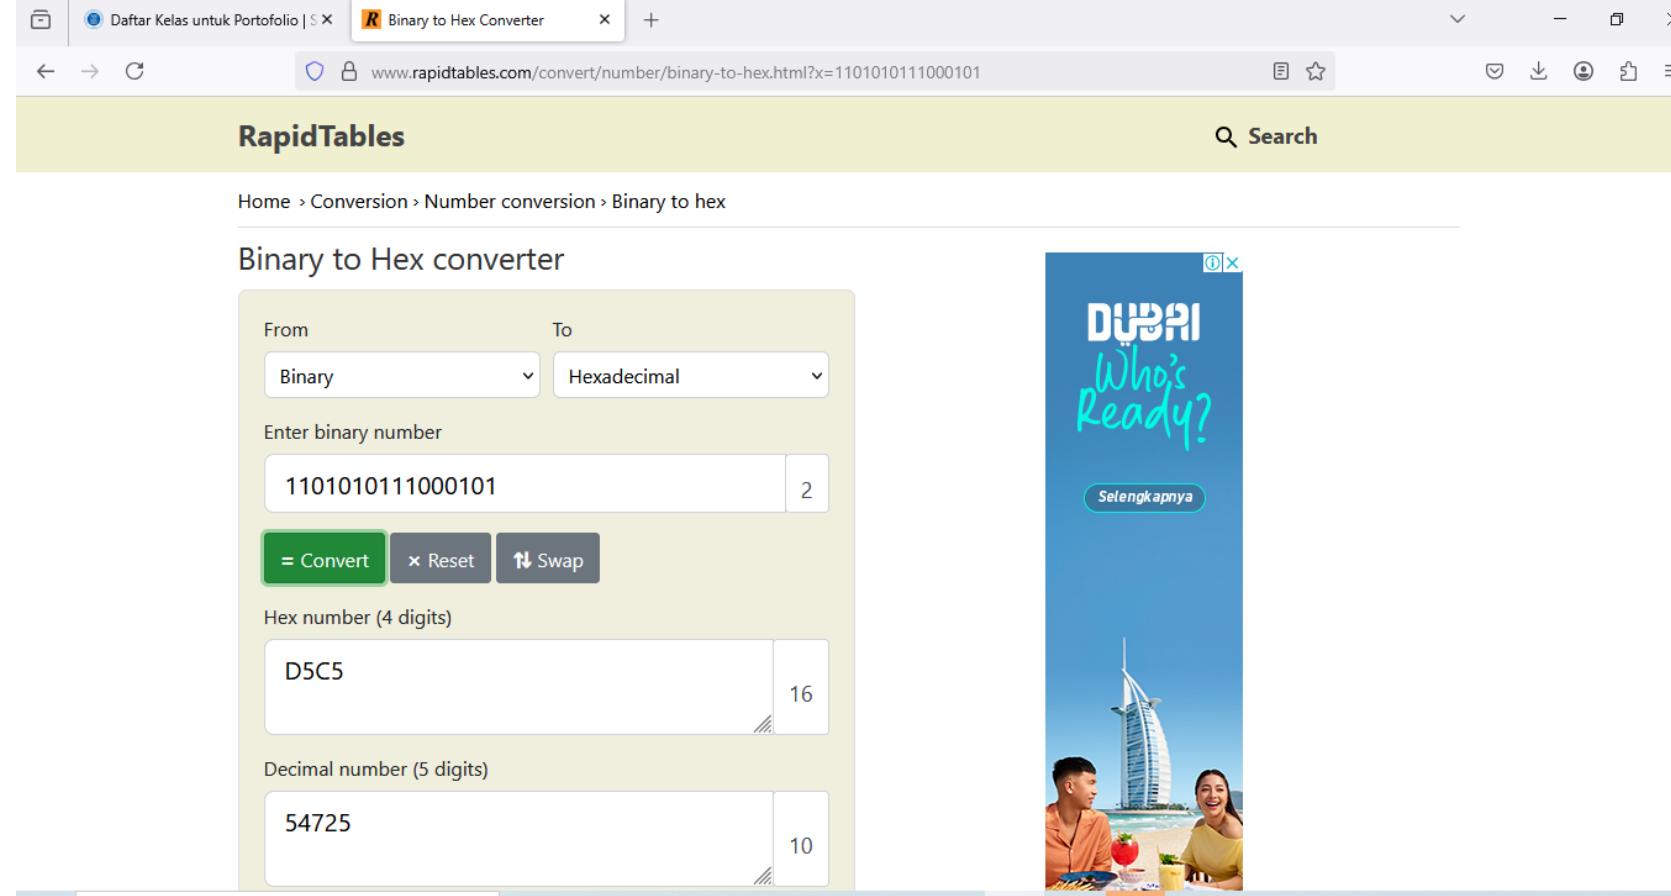
\includegraphics[width=182.70mm,height=246.51mm]{../../images/llm/page_008_img_01.png}%
\end{textblock*}

\end{document}
